% -----------------------------------------------
% Template for ISMIR 2010
% (based on earlier ISMIR templates)
% -----------------------------------------------

\documentclass{article}
\usepackage{ismir2010,amsmath,cite}
\usepackage{graphicx}
\usepackage{url}
\usepackage{algorithm,algorithmic}


% Title.
% ------
\title{Large-scale harmonic patterns clustering}

% Single address
% To use with only one author or several with the same address
% ---------------
%\oneauthor
% {Names should be omitted for double-blind reviewing}
% {Affiliations should be omitted for double-blind reviewing}

% Two addresses
% --------------
%\twoauthors
%  {First author} {School \\ Department}
%  {Second author} {Company \\ Address}

% Three addresses
% --------------
\threeauthors
  {First author} {Affiliation1 \\ {\tt author1@ismir.edu}}
  {Second author} {\bf Retain these fake authors in\\\bf submission to preserve the formatting}
  {Third author} {Affiliation3 \\ {\tt author3@ismir.edu}}
% what order do we use? Thierry, Ron, Dan? is Graham on?


\begin{document}
%
\maketitle
%
\begin{abstract}
We present a method for discovering typical patterns in music.
Following up on the \textit{Shingle} idea, we bring these harmonic patterns
into the clustering framework. We use EchoNest API and a training set
of $43$K songs to assert our method. We restrain ourselves to an online
algorithm, thus it can scale to arbitrary data sizes.
We assess the basic good behaviours of our algorithm on this harmonic
data. We explain how to interpret the centroids of the clusters through
visualization and further encoding. We discuss ways to move to even larger
scales and we provide our code for reproducing the results.
TAKE-HOME MESSAGE: \textit{Shingles} idea can go large-scale?
\end{abstract}
%
\section{Introduction}\label{sec:introduction}

Working with large amount of audio data is a goal and a challenge at the
same time. One of the most common task is to find the nearest neighbor,
based on some distance, to a given segment of music. This can be viewed
as \textit{retrieval} as you are looking for some specific target
based on some query. $k$-nearest neighbors ($k$nn) algorithms have been
designed for that purpose, and recent improvements let them scale to
considerable data set sizes \cite{Datar2004}. The \textit{Shingles}
were introduced in that framework \cite{Casey2006}. A \textit{Shingle}
is a pattern of stacked chroma features. Similarity between
\textit{Shingles} coresponds to similarity between harmonic patterns. For this
reason, they were used for cover or remix recognition \cite{Casey2007}.

That being said, nearest neighbor search is only one aspect of the
analysis of large-scale music data sets. Finding $k$ neighbors for a
particular query does not tell you much about the music space.
Clustering is a larger and more flexible framework where the goal is
to divide the space in meaningful blocks. The starting point is not
a query, but all the data itself. In this work, we bring the
\textit{Shingle} idea into that framework in order to discover
meaningful and typical music harmonic patterns. The underlying assumption
is that the music space is articulated around a certain number of
frequent patterns.

Note that clustering and neighbor search are not unrelated.
In practise, we would hope that close neighbors live in one or two
close clusters, thus clustering can be a preprocess step. Also,
knowing all $k$ neighbors of each sample let you do graph clustering,
a subset of the clustering algorithms.

We investigate a vector quantization \cite{Datar2004} (VQ) method to
cluster the \textit{Shingles}. We create a codebook of typical patterns
that have many usages:
\begin{enumerate}
\item describing the music space
\item finding potential similar songs and/or covers
\item eliminating quickly very wrong matches in a query system
\end{enumerate}


A major component of this work is scalability. We experiment with a training
set of $43$ thousands song, but everything scales linear in time
relative to the number of samples. We could imagine, as an extension
of this work, an algorithm ``listening'' to all music it can find online.
Training time would be an issue, but not memory.


In this paper, we present a practical way to do such large-scale 
clustering using online vector quantization. We present clustering results 
of an online algorithm on a data set of $43$K songs, but the method applies 
to any data size. We show how to select different parameters such as the size 
of the \textit{Shingles} using an encoding scheme on a test set of $8$K songs. 
Finally, we illustrate the method with some specific examples.



\subsection{Definitions}
A pattern, or a patch, is a \textit{Shingle} taken from an actual song.
A code is similar to a pattern, but is the result of the clustering
algorithm and most likely does not come from an actual song.
Distortion is our measure of distance between a pattern and a code
(or between two patterns, see equation \ref{eq:dist} in Section 
\ref{sec:experiments}).


\section{Previous Work}\label{sec:prevwork}
Our work can be seen as an extension of the \textit{Shingles} idea
described by Casey and Slaney \cite{Casey2006,Casey2007,Casey2008}.
The two main differences are the clustering framework and the use of
beats and bars to select the position of the \textit{Shingles}.

Casey and Slaney \cite{Casey2006} use LSH \cite{Datar2004} to perform
fast approximate nearest neighbor search. Their implementation is E$^2$LSH
\cite{E2LSH}. This package can efficiently handle about $50$K or $100$K
vectors of size $200$. Even with a better implementation, the LSH
model still has some scaling problem. A large portion of the data
must be known to decide how many projections to use, and what guarantee
of finding the nearest neighbor it can provides. Also, we could fix the
number of projections and consider as clusters all the elements that
fall into the same bin. However, this does not give us a centroid, a
typical pattern representing that cluster.

Nearest neighbor and clustering methods are common in music similarity 
research, for instance \cite{Cano2004,Holzapfel2009}. The difference here 
are the actual patterns that we cluster.

Regarding similar representations of music,
Barrington et al. recently studied music texture using a set of ordered
MFCC vectors \cite{Barrington2009a}. This could be seen as complementary
to our work. Chromas capture the harmonic information and some of the
rythm while the MFCC are great timbral features.

Other large-scale work use summarization of the features. We mention 
gaussian mixtures \cite{Mandel2005}, 
aggregate features \cite{Bertin-Mahieux2008}
and linear dynamical systems \cite{Barrington2009a}. 
The advantage of \textit{Shingles} representation (stacked chroma vectors)
is that it is close from an harmonic point of view to the actual music, 
in particular
we can ``listen'' to the patches (see Section \ref{sec:experiments}).
This is an advantage for analyzing a large data set, thus
we restrain ourselves from using generative models to compress our features.


\section{Data}\label{sec:data}
In this section we present our use of the Echo Nest features and the
datasets we use for training and testing our model.


\subsection{Echo Nest features}
We use the Echo Nest analyze API \cite{EchoNest} throughout this work.
The API gives us a chroma vector (length $12$) for every music event, 
or ``segment'', for any song we upload to their platform. 
We also get an estimate of where the beats and the bars are. Beats span over
multiple segments, and bars span over multiple beats. 
We transform the chroma vectors per segment into per beat vectors using a 
simple average. We can then stack beat vectors for a number of bars 
(usually 1 or 2). 
We get a fixed-size patch by resampling the number of chroma vectors. Typically,
there are $4$ beats per bar. Thus an appropriate pattern size for one bar
is $12$x$4$ or $12$x$8$.

Note that we do not claim that any of these informations (segments, beats, bars)
are perfectly accurate (e.g. in \cite{Barrington2009a} authors obtain a better
song segmentation than Echonest). Practise showed us that they are reasonable, 
and the size of the data set should make up for the imperfections or noise.
We also believe that patches sizes based on a number of beats or bars are more
meaningful than an arbitrary time length. More on this in the experiments
(Section \ref{sec:experiments}).


\begin{figure}[htb]
\begin{center}
\includegraphics[width=.8\columnwidth]{code}
\end{center}
\caption{{A typical code from a codebook of size $200$. Patterns represented
$2$ bars and the pattern length was set to $16$.}}
\label{fig:code}
\end{figure}

\subsection{Cowbell Dataset}
We have $43,300$ songs, giving  $3,720,091$ non zero bars, a bar usually 
contains $4$ beats. WHERE DOES THIS DATA COMES FROM? GIFT FROM EN?


\subsection{uspop2002}
We had acces to a low quality (32kbps) version of the songs in the uspop 2002 
data set \cite{uspop2002}.
This well-known data show a great diversity of pop songs, but is not particular
otherwise. We also tried to use Tzanetakis dataset \cite{Tzanetakis2002a}, but 
the $30$ seconds segments seemed hard to analyze by the Echo Nest API, most did
not contain any bar.

uspop2002 serves as testing set to measure how well a codebook learned on
the Cowbell data set can represent new songs. We get Echo Nest features
for $8651$ songs from that dataset.

\section{Algorithm}\label{sec:algo}
In this section we present the creation of the harmonic patterns from
the Echo Nest data. Then, we explain the online vector quantization algorithm
used to learn a codebook of those patterns.

\subsection{Pattern Creation}
Here we should explain key invariance, resizing, etc, and not in the
experiment section.

We try to normalize the patterns in respect to the key. We roll the matrix
so the row with the more energy is always the lowest one. This can easily be
seen in Figure \ref{fig:code}. We considered the same technique for rolling
along the other axis and be invariant regarding the downbeat. However, it
seems less robust to noise. Note that we roll each pattern independentely.
Also, this implies that the pitch envelope is important rather than the actual 
pitches.



\subsection{Codebook Learning}
We use an online version of the vector quantization algorithm 
\cite{Gersho1991}. This can also be seen as an online K-means.
The idea is as follow: take a sample from your data, find the closest
code in the codebook, bring that code closer to the sample by some amount.
The details are explained in Algorithm \ref{algo:vq}. Note that this
algorithm, though not optimal, is $O(n)$ with $n$ number of songs seen.
Thus it scales linearly to any size of data set. The setting of the learning
rate might become trickier, but this is not fundamentally a problem.


We initialize the codebook by choosing $K$ random points from our dataset.


\begin{algorithm}
%\caption{Pseudocode of Vector Quantization}
\begin{algorithmic}
\STATE$l$ learning rate
\STATE$\{P_n\}$ set of patches
\STATE$\{C_k\}$ codebook of $K$ codes
%\STATE $m \leftarrow b$
\REQUIRE $0 < l \leq 1$
\FOR{$nIters$}
\FOR{$p \in \{P_n\}$}
\STATE$c \leftarrow min_{c \in C_k} dist(p,c)$
\STATE$c \leftarrow c + (p - c) * l$
\ENDFOR
\ENDFOR
\RETURN $\{C_k\}$
\caption{{Pseudocode of Online Vector Quantization. Note that we can replace
the number of iteration by a threshold on the distortion over some test set.}
\label{algo:vq}}
\end{algorithmic}
\end{algorithm}






\section{Experiments}\label{sec:experiments}
In this section we present general experiments that describe our method.
We start by giving some details on how we selected our training set and
how to measure error. Secondly, we experiment with different pattern sizes.
Thirdly, we look at the effect of the size of the
data set on the training. The next experiment look at the size of the
codebook. Then, we show that the patterns are not random,
which is expected from music data. Finally, we show examples of patterns,
codebooks and clusters.


\subsection{Setting}\label{ssec:setting}
We take one or two bars, normalize the patches to size 4, 8, or 16.
We roll the patch to be invariant to the key (on the patch level, not on
the song level). We learn a codebook of size $K$ over the cowbell dataset 
using the VQ algorithm (Algorithm \ref{algo:vq}). A typical learning rate 
is $0.01$ for $20$ iterations over the whole dataset.

We use the codebook to encode our testing set (see Section \ref{sec:data}).
Each pattern is encoded with only one code. We can measure the average
distance between a pattern and its encoding. We can also measure the use
of the different codes, i.e. the size of the cluster around a code.

As a distance measure (or distortion measure) between patterns, we use
the average squared euclidean distance. In details, if a pattern $p1$
is composed of elements $p1_{i,j}$, and similarly for a pattern $p2$,
the distance between $p1$ and $p2$ is:
\begin{eqnarray}
  dist(p1,p2) = \sum_{i,j} (p1_{i,j} - p2_{i,j})^2 / size(p1)  \label{eq:dist}
\end{eqnarray}
We assume $p1$ and $p2$ have the same size.

\subsection{Pattern length}
See encoding experiments in Table \ref{tab:psize}.


% RESULTS
% 200codes, 2 bars, pSize=16, maxener, True, False, not scaled = 
% 200codes, 2 bars, pSize=8, maxener, True, False, not scaled  = 0.042432
% 200codes, 1 bars, pSize=4, maxener, True, False, not scaled  = 
% 200codes, 7 beats, pSize=7, maxener, True, False, not scaled = 
% 200codes, 5 beats, pSize=5, maxener, True, False, not scaled = 
% 200codes, 3 beats, pSize=3, maxener, True, False, not scaled = 
\begin{table}
\begin{center}
\begin{tabular}{|l|c|}
\hline
size & avg. dist \\ \hline \hline
1 bar (4) & $0.036722$\\
2 bars (8) & $0.044301$\\
2 bars (12) & $0.043583$\\
2 bars (16) & $0.044086$ \\ \hline
3 beats & $0.032688$\\
5 beats & $0.040858$\\
7 beats & $0.045515$\\ \hline
\end{tabular}
\end{center}
\caption{{Encoding score for different pattern sizes. We can select the
size of the patterns based on bars. In this case, we put the actual size
of the pattern in parentheses. If the pattern size is based on beats, the
size is the number of beats. Results are on the uspop dataset, not seen
during training.}}
\label{tab:psize}
\end{table}


\subsection{Data Size}
We are interesting to see how the amount of training data changes
the quality of our codebook.
We experiment with different data sizes for a fixed size of codebook and a 
fixed code length. The data points are chose randomly from the whole
data set.
In the experiment a pattern size correspond to $1$ bar resized to $4$
beats, thus a pattern size of $12$x$4$. The codebook size is $100$.
We measure the distortion on our test set. 
See results in Figure \ref{fig:sizes}.

Our learning can overfit, which explain the bad scores of small datasets.
The larger the dataset, the smallest the chance to overfit.
We are looking for a size of dataset that guarantees us a good learning
process, while being unnecessary large.

$500$ samples per code in the codebook seems a good data size, see
Figure \ref{fig:sizes} for size $50$K.

\begin{figure}[htb]
\begin{center}
\includegraphics[width=.99\columnwidth]{data_sizes}
\end{center}
\caption{{Distortion for a codebook of size $100$ encoding one bar
at a time, a bar being represented by $4$ chroma feature vector.
Therefore, a code or a pattern is of size $12$ x $4$ = $48$.
Distortion measure on the test data set. Data size tested range
from $10$ thousands to $2$ millions. Patterns were selected at
random from the dataset of approximately $3,7$ million patterns.}}
\label{fig:sizes}
\end{figure}

\iffalse
\begin{table}
\begin{center}
\begin{tabular}{|l|c|c|c|c|c|c|}
\hline
size & $5$K & $10$K & $50$K & $100$K & $500$K & $2$M  \\ \hline
distortion & $$ & $0.143$ & $0.142$ & $0.142$ & $0.142$ & $$\\ \hline
\end{tabular}
\end{center}
\caption{{Distortion for a codebook of size $100$ encoding one bar
at a time, a bar being represented by $4$ chroma feature vector.
Therefore, a code or a pattern is of size $12$ x $4$ = $48$.
Distortion measure on the test data set. Data size tested range
from $10$ thousands to $2$ millions. Patterns were selected at
random from the dataset of approximately $3,7$ million patterns.}}
\label{tab:datasize}
\end{table}
\fi
% RESULTS:    
% 1bar s4     avg_distOLD    avg_dist
% 1K          0.150370       0.041941
% 5K          0.145327       0.038449
% 10K         0.143567       0.036892
% 50K         0.142257       0.036722
% 100K        0.142195       0.035973
% 250K        0.141796       0.035910
% 500K        0.142081       0.035904
% 1M          0.142118
% 2M          0.141596
% 1bar s4 first X samples
% 1K          0.157142       
% 5K          0.150045
% 10K         0.148357
% 50K         0.146069
% 100K        0.145765
% 250K        0.145819
% 500K        0.145772
% 1M          0.145924
% 2M          0.146065       
% 0bar s4 (and test set same, we could do 1bar s4 in test set...)
% 1K          0.155474       0.042596
% 5K          0.149619       0.038971
% 10K         0.148056       0.038114
% 50K         0.146328       0.037181
% 100K        0.146004       0.037055
% 250K        0.146024       0.037014
% 500K        0.145962       0.037004
% 1M          0.145873
% 2M          0.145955
% 2bar s8     
% 1K          0.171300       0.049282
% 5K          0.165960       0.046441
% 10K         0.165063       0.045507
% 50K         0.162439       0.044301
% 100K        0.161588       0.044183
% 250K        0.161910       0.043896
% 500K        0.161233       0.043906
% 1M          0.161057
% 2M          0.161068


\subsection{Codebook Size}
We experiment with the size of the codebook and its affect on the
performance of the encoding. Results are shown in Table \ref{tab:cbsize}.
Note that we trained on a number of samples depending on the codebook
size, i.e. we used $500$ samples per code to learn. This is consistent
with our findings from Figure \ref{fig:sizes}.


\begin{table}
\begin{center}
\begin{tabular}{|l|l|c|}
\hline
\# codes & \# samples & avg. dist \\ \hline \hline
1 & $500$ & $0.066079$ \\
10 & $5$K & $0.045690$ \\
50 & $25$K & $0.038456$ \\
100 & $50$K & $0.036725$ \\
200 & $100$K & $0.033923$ \\
500 & $250$K & $0.030973$ \\
1000 & $500$K & \\ \hline
\end{tabular}
\end{center}
\caption{{Experiment with the codebook size. We train on patterns
corresponding to $1$ bar resized to $4$ beats. The number of training
samples is set to $500$ times the number of codes, which is sufficient
according to Figure \ref{fig:sizes}.}}
\label{tab:cbsize}
\end{table}
% RESULTS:      avg_distsOLD    avg_dist
% code 1        0.195939        0.066079
% code 10       0.161812        0.045690
% code 50       0.147472        0.038456
% code 100      0.142194        0.036725
% code 200      0.137548        0.033923
% code 500      0.131211        0.030973
% REDONE WITH FIX NUMBER OF FEATURES - 500K (new correct dist)
% code 1        
% code 10       0.045579
% code 50       0.038302
% code 100      
% code 200      
% code 500      


\subsection{Codebook Size in Function of Pattern Length}
We experiment on the randomness of the \textit{Shingles}, assuming
that there is some correlation between beats and bars.
The intuition is as follow: if the signal was totally random, every
time the signal size double, the codebook size must be squared.
To illustrate this, imagine a binary array of length $1$. We need two
codes to encode perfectly: $(0)$ and $(1)$. If the binary array is now of
length $2$, we need four codes: $(0,0)$, $(0,1)$, $(1,1)$ and $(1,0)$.

In Table \ref{tab:size_pattern}, we test that hypothesis. As expected,
the distortion improves with larger pattern sizes. The details
are difficult to analyze. The error jump from two beats to one bar
can probably be explained by the obvious case of sustained notes.
We also believe that smaller codebooks are more affected by their
initialization. Fortunately, we can conclude that music is not random,
which is always a good sanity check!


Then... 3 beats, 5 beats, 7 beats don't encode as well?

Special: 4 beats versus 1 bar - 4 beats, show the problem of being
not in sync with bars.

See codebook size experiments in Table \ref{tab:cbsize}.

\begin{table}
\begin{center}
\begin{tabular}{|l|c|c|}
\hline
\# codes & \# bars & avg. dist \\ \hline \hline
2 & $1$ & $0.058435$ \\
4 & $2$ & $0.054792$ \\
16 & $4$ & $0.055489$ \\
256 & $8$ & $0.054860$ \\ \hline
2 & $2$ beats* & $0.066416$ \\
4 & $1$ & $0.050712$ \\
16 & $2$ & $0.050172$ \\
256 & $4$ & $0.049894$ \\ \hline
\end{tabular}
\end{center}
\caption{{Codebook size in function of the number of bars to encode.
All experiments done wtih $256 \times 500 = 128$K samples randomly chosen.
* For the $2$ beats experiment, we take the first half of every beats.
It is different from ignoring bars and taking every $2$ beats. It is more
coherent with the other settings ($1-2-4-8$ bars).}}
\label{tab:size_pattern}
\end{table}
% RESULTS:           avg_distsOLD   avg_dist
%2 codes 1 bar       0.180750       0.058435
%4 codes 2 bars      0.183631       0.054792
%16 codes 4 bars     0.184078       0.055489
%256 codes 8 bars    0.183464       0.054860
%---------------
%2 codes 2 beats     0.166840       0.046955
%2 codes 2 beats                    0.066416
% based on bars
%4 codes 1 bar       0.171495       0.050712
%16 codes 2 bars     0.173767       0.050172
%256 codes 4 bars    0.174169       0.049894


% see generate_expo_codes_curves.py to generate the following figure:
\begin{figure}[htb]
\begin{center}
\includegraphics[width=.99\columnwidth]{codesize_patternsize}
\end{center}
\caption{{Possible figure to replace Table \ref{tab:size_pattern}.}}
\label{fig:size_pattern}
\end{figure}


\subsection{Bar offset}
We study how great are patterns based on bars by playing with an offset.
The offset can be $0$ (normal case) or a quarter of bar, half a bar, and
three quarters of a bar.

\begin{table}
\begin{center}
\begin{tabular}{|l|c|c|}
\hline
offset & avg. dist \\ \hline \hline
$0$ & $$ \\
$.25$ & $$ \\
$.50$ & $$ \\
$.75$ & $$ \\
\end{tabular}
\end{center}
\caption{{Results with different offset. Always $100$ codes.
\label{tab:offset}}}
\end{table}
% RESULTS             avg_results
% 0 offset
% .25 ofset           0.037130
% .50 ofset           0.037241
% .75 ofset           0.037337
% RESULTS FOR PARTIALBAR TOO
% 0 off .25 part      0.046304
% .25 off .25 part    0.044950
% .50 off .25 part    0.044395
% .75 off .25 part    0.044473




\subsection{Visualization}
Interpreting a codebook of size larger than $100$ is not obvious.
We can use an algorithm like locally linear embedding \cite{Roweis2000} (LLE) 
or multidimensional scaling \cite{Kruskal1964} to visualize the data in
2 dimensions. Here we use the former\footnote{implementation: 
\url{http://www.astro.washington.edu/users/vanderplas/coding/LLE/}}, the
result can be seen in Figure \ref{fig:lle}.


\begin{figure}[htb]
\begin{center}
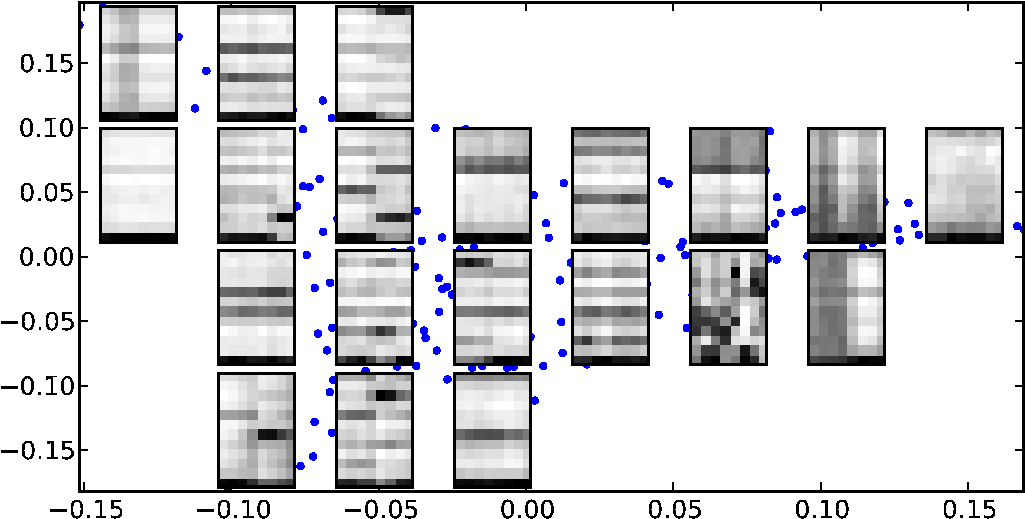
\includegraphics[width=.9\columnwidth]{codes_lle}
\end{center}
\caption{{LLE visualization of the codebook.}}
\label{fig:lle}
\end{figure}

Another way is simply to present the codes in order of cluster size.
We encode the training or testing set as explained in Subsection 
\ref{ssec:setting} and we count how many patterns were closer to a particular
code than any other code. In Figure \ref{fig:firstcodes}, we show the $25$
most used codes out of a codebook of size $200$.
Code from Figure \ref{fig:code} is the 37th most used code in that
codebook. In Figure \ref{fig:closep}, we show a sample of patterns that
fall into its cluster.


\begin{figure}[htb]
\begin{center}
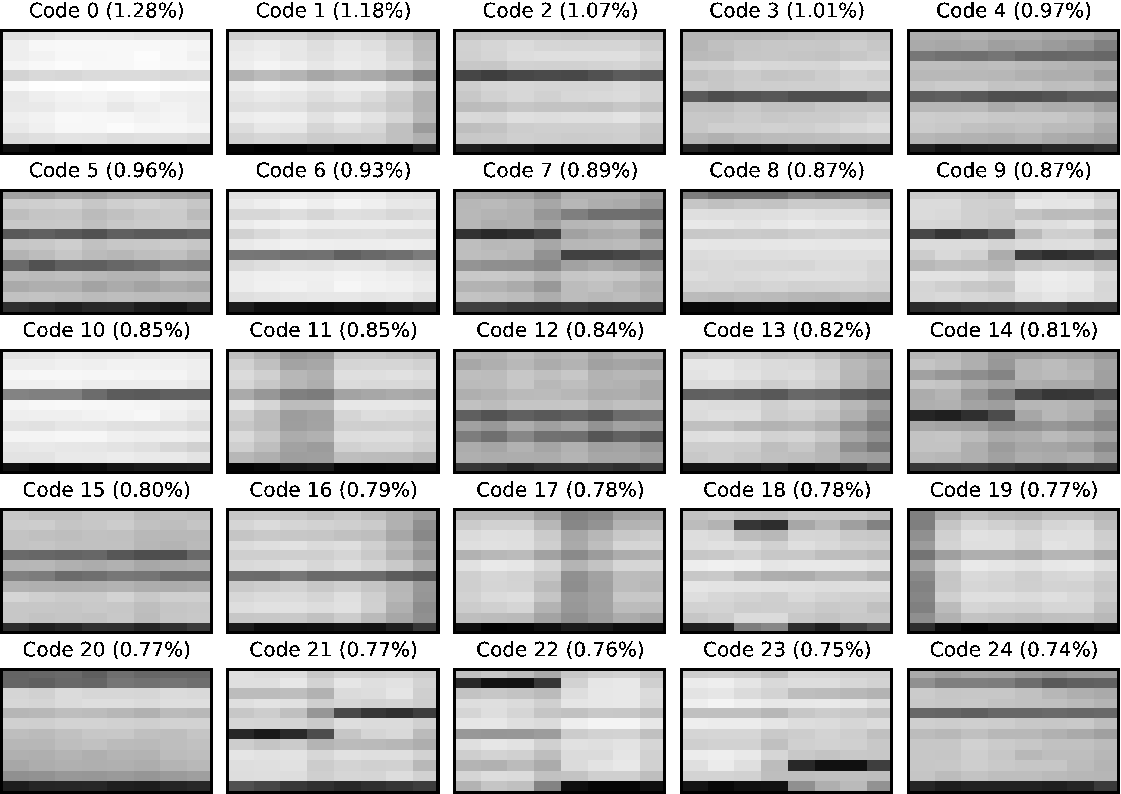
\includegraphics[width=.9\columnwidth]{codes1}
\end{center}
\caption{{$25$ most used codes on the training set.}}
\label{fig:firstcodes}
\end{figure}

The most common pattern is a sustained note, as we can see in Figure
\ref{fig:firstcodes}. Another common pattern is a sustained note
with an harmonic, as seen in the LLE visualization (Figure \ref{fig:lle}).

\begin{figure}[htb]
\begin{center}
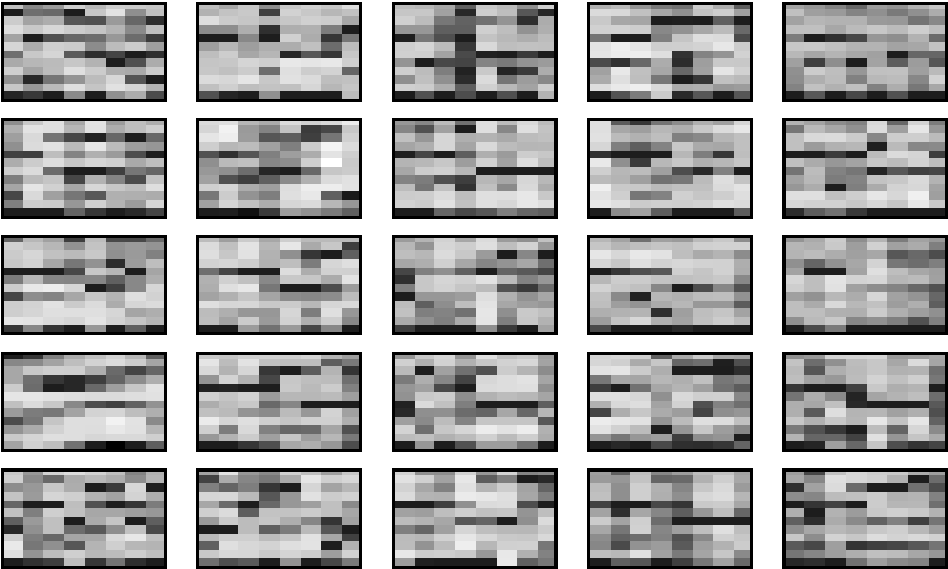
\includegraphics[width=.9\columnwidth]{close_patterns1}
\end{center}
\caption{{Sample of the close patterns to code in Figure \ref{fig:code}.}}
\label{fig:closep}
\end{figure}

\subsection{Specific Examples}


\section{Links with NMF}\label{sec:nmf}
In this section we discuss links with non-negative matrix factorization
\cite{Lee2000} (NMF), another method to build a codebook representing some data.
NMF finds two matrices $H$ and $W$ that approximate some data $D$ (one
sample per line) by
\begin{eqnarray}
D \approx W^{m \times k} H^{k \times n}
\end{eqnarray}
where $\epsilon$ is some noise and $W$ and $H$ only have non-negative 
elements. If $W$ is $\#samples \times k$, $k$ is the codebook size.

Note that NMF does not solve the same problem. It tries to explain each pattern
as a combination of codes. Thus it does not perform clustering, though you
could cluster patterns using their encoding weights. Also, we do not fully
compare our methods with NMF, it would be a paper on its own.

In all our experiments we use the following NMF
implementation\footnote{implementation: \url{http://www.ee.columbia.edu/~grindlay/code.html}}.

\subsection{Training NMF on our Codebook}
NMF provides us with a way of measuring how much information is retained
in our codebook. More specifically, we can train a codebook of size $500$
using our online VQ algorithm, then decompose that code into $10$ basis
using NMF. We can compare that to $10$ basis from training NMF on the
whole data.

The idea is simple, if we encode our test set using basis from the
codebook as well as if we were using basis from the whole data, our codes
retain much of the information. That being said, the typical NMF implementations
are not expected to scale to data that does not fit in memory. Online VQ
could be an interesting preprocessing step. Future work include looking
at online NMF \cite{Thurau2009}.

\subsection{Experiment}
Put figure, compare basis, yeah!

\begin{table}
\begin{center}
\begin{tabular}{|l|l|c|c||c|}
\hline
\# codes & \# bars & full data & codebook & test set \\ \hline \hline
10 & 1 & $$ & $$ & \\ \hline
20 & 1 & $$ & $$ & \\ \hline
10 & 2 & $\bf{1774788}$ & $$ & $1782164$\\ \hline
20 & 2 & $$ & $$ & \\ \hline
\end{tabular}
\end{center}
\caption{{Encoding error of the test data set using NMF basis learned
on the whole data and on the codebook. We also encode the test set
directly to give us an upper bound.}}
\label{tab:nmf}
\end{table}
% RESULTS:         whole data             codebook     test set
%10 codes 2 bars   1774788.2566 (200 it)               1739639.7304 (1000 it)
%10 codes 1 bar


\section{Conclusion}
We presented a practical method to perform large-scale clustering of
harmonic patterns. We assessed the basic properties of the method through
experiments on a large collection of music. We suggested many ways
to interpret the data through visualization (LLE) and further encoding
(NMF). We discussed the possibility to move to even larger scales
and we provided our source code\footnote{Code not yet released to preserve
submission's anonymity}.

As for enhancements, we specifically did not compress our features using
gaussian mixtures or other generative model. That being said, these methods
could be use to develop better distance measures between \textit{Shingles}.
The use of the euclidean distance is arbitrary. Summarizing patches
with gaussians, and then comparing the distance between those gaussians,
could reduce the influence of the noise in the distance measure.

Moving on to larger scales, we could imagine merging codes together and
splitting some on two if the clusters become too small or too large.We could
also cluster the codebook itself, in a similar fashion as hierarchical
gaussian mixtures \cite{Vasconcelos2001}.


\small
%\section{Acknowledgements}
%Thierry is NSERC graduate fellow, or some title like that.
% Graham for the NMF stuff, unless is an author.

%\begin{thebibliography}{citations}
%\bibitem{Someone:04} 
%X. Someone and Y. Someone:
%{\it Title of the Book},
%Editorial Acme, Utrecht, 2004.
%\end{thebibliography}

\bibliography{tbm_bib}





\end{document}
